\documentclass[oneside]{article}

\usepackage[margin=1in]{geometry}
\usepackage{mathpazo,graphicx,hyperref}

\hypersetup{
  colorlinks   = true, %Colours links instead of ugly boxes
  urlcolor     = blue, %Colour for external hyperlinks
  linkcolor    = blue, %Colour of internal links
  citecolor   = red %Colour of citations
}

\begin{document}
\title{Milestone 2}
\author{Guillaume Labranche \and William Bain \and Si Mei Zhang}
\maketitle

\tableofcontents

\section{Design decisions}

\subsection{Typechecker}

In accordance with the instructions our type checking is executed in a single pass without forward declaration.\footnote{See \url{https://mycourses2.mcgill.ca/d2l/le/161312/discussions/threads/258597/View}.} We are working in Java and we implemented the typechecker as a subclass of the \verb|DepthFirstAdapter| class provided by SableCC. This made it easy to traverse the AST without extra boilerplate. Since we did not have a reliable way of editing the extending the AST classes generated by SableCC, we stored type information for the AST in a hash table mapping from nodes to Go types.\footnote{By extending I mean adding methods and properties to a class used by the parser (here probably \texttt{PExp}, the abstract expression production class), not just creating a subclass.}

In most cases it was sufficient to apply typechecks after the the typechecker had recursed over the child nodes and typechecked them. There were two cases where more fine-grained control was necessary:

\begin{itemize}
    \item In short assignment statements, the list of variables is implemented as a list of expressions for reasons having to do with the parser implementation. It was therefore necessary to stop the typechecker from typechecking the variables before they had been added to the symbol table.
    \item To typecheck function declarations and if statements, it was necessary to open a scope after having typechecked some but not all of the child nodes.
\end{itemize}

In each of these special cases we overrode the \verb|case| method which controls the recursion over the child nodes.

A further implementation detail that is worth noting is our implementation of struct type declarations. To prevent code duplication, we treat struct fields as if they were variable declarations: we open a scope in the symbol table upon entering the struct and enter each field as if it were a variable. Then we pop the scope and use it to build the struct class.

\subsection{Symbol table}

Initially the symbol table was simply a scope with a reference to the parent scope. Traversing up and down the scopes meant overwriting the variable used to reference the scope, so we decided to make \texttt{SymbolTable} be what its name suggests, and take care of scoping up and down. It holds a double-ended queue (Java's \texttt{ArrayDeque}) to store the scopes. We have methods for different use cases: searching for an identifier through all scope levels, and searching only in the current scope.

We have also added loggers to enable the \verb|-dumpsymtab| and \verb|-dumpsymtaball| CLI options.

\subsection{Type and symbol class hierarchy}

We put considerable effort into developing and revising the hierarchy representing GoLite types and symbols (figure \ref{fig:symbol_table_uml}). We adopted the following goals, listed here roughly in descending order of precedence:

\begin{enumerate}
    \item Type safety: as much as possible, it should not be possible to use an object in a place where it is not allowed. This should be detected at compile time.
    \item Simplicity: there should not be more classes or objects than are necessary. For instance, we did not want to use a class \texttt{AliasTypeSymbol(Symbol s)} to wrap every type alias entered in the symbol table.
    \item DRY: it should not be necessary to implement functionality in multiple places.
\end{enumerate}

\begin{figure}
    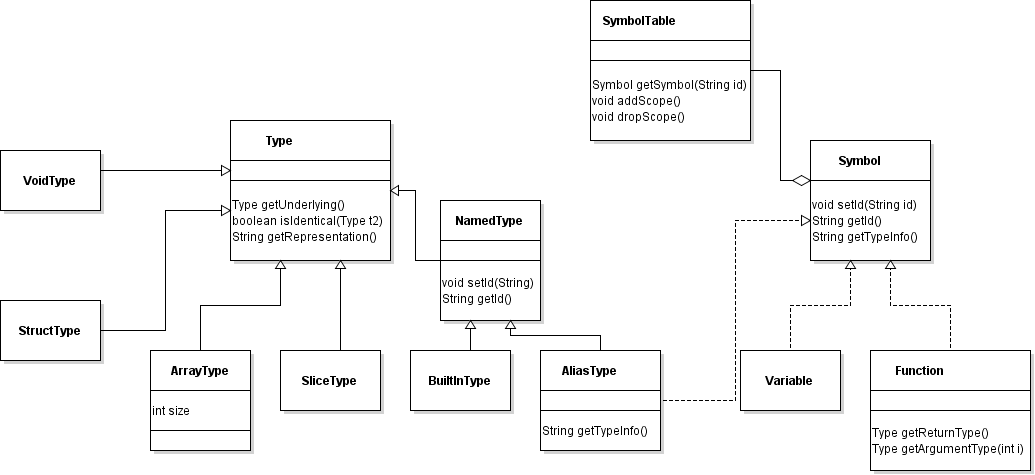
\includegraphics[width=\textwidth]{symbol_table_uml}
    \caption{Class hierarchy for GoLite types and symbols (property and method listings are non-exhaustive)}
    \label{fig:symbol_table_uml}
\end{figure}

These considerations led us to a number of particular decisions. First, we place functions outside the type hierarchy. While in Go functions are first class citizens, with their type given by the function signature, in GoLite they are not. Therefore, instead of implementing functions as instances of \texttt{Variable}, which would potentially allow them to be used where another objects of another type are required, we implemented a \texttt{Function} class which represents a particular function and stores both the function's identifier and its associated type information directly.

Second, we made \texttt{Symbol} an interface which is implemented by the \texttt{Variable}, \texttt{Function}, and \texttt{AliasType} classes. The difficulty here was that since \texttt{AliasType} is a subclass of \texttt{Type}, it could not also inherit from an abstract \texttt{Symbol} class. By making \texttt{Symbol} an interface, we allow \texttt{AliasType} instances into the symbol table directly without thereby making it possible to enter other types---for instance the \texttt{BuiltInType} which we use for \texttt{int}, \texttt{bool}, \texttt{alias}, and \texttt{rune}---illicitly. The downside of this design is that the \texttt{getId} and \texttt{setId} methods required by \texttt{Symbol} had to be implemented at least twice. However, this was sufficiently trivial that it did not change our decision. In fact, the duplication is so trivial that we did not even create a shared superclass for \texttt{Function} and \texttt{Variable} to reduce the duplication there.\footnote{We \emph{did}, however, create a \texttt{NamedType} class which is extended by both \texttt{BuiltInType} and \texttt{AliasType}. This class also implements the \texttt{isIdentical} and \texttt{getRepresentation} methods.}

A final decision worth noting is our use of the \texttt{VoidType} class. Since unfortunately Java does not make it possible to statically forbid null pointers, it is easy to introduce them accidentally. To help catch such cases, we use \texttt{VoidType} instead of \texttt{null} to represent the return type of a function that does not return a value.

\subsection{Typed pretty printer}

We extended the \verb|PrettyPrinter| class we implemented in Milestone 1 to have it print extra type information. By overriding the \verb|defaultOut| method, it was simple to have it look up and output the type of any node which is an instance of the \verb|PExp| (expression production) class as an inline comment.

\section{Scoping rules}

The scoping rules are in accordance with the GoLite specifications:

\begin{itemize}
    \item In a given scope, it is legal to refer to an identifier that was previously declared in the scope or one of the parent scopes.
    \item It is illegal to declare a new type, variable or function using an identifier previously defined in the current scope only.
    \item The following language structures create new scopes for themselves: \texttt{if}, \texttt{else}, \texttt{for}, \texttt{func}, \texttt{struct}, standalone block (\verb|{...}|). The if and else branches of the if statement also create their own scopes.
\end{itemize}

\section{Type check operations}

TODO description and concordance

In some cases there are multiple code paths which lead to the same error. For instance, the helper method \texttt{ensureUndeclared(TId id)} is called in a number of places to ensure that an identifier has not previously been declared in the current scope. While we have done fuzz testing, we have not created an exhaustive suite of failing programs to cover each possible path to the error in such cases.

\subsection{General}

\begin{description}
  \item[Use of undefined variable:] \verb|identifier_undefined_in_symtab.go|, \verb|append_id_undefined.go|
  \item[Redeclaration of variable in same scope:] \verb|redeclaration_of_var_in_same_scope.go|
  \item[Mismatching types in binary operation:] Generic check that operands share the same type. \verb|binary_op_mismatch.go|, \verb|assign_op.go|
  \item[Mismatching types in op-assign statement:] Check that operands are of a type the operation supports. \verb|field_selection_id_mismatched.go|
\end{description}

\subsection{Toplevel declarations}

\subsection{Statements}

\subsubsection{Assignment}
\begin{description}
  \item[Assignment to a variable with different underlying basic type:] \verb|use_different_type_in_assignment.go|
\end{description}

\subsubsection{Op assignment}
\begin{description}
  \item ***
\end{description}

\subsubsection{Increment/decrement statement}
***

\subsubsection{Short variable declaration}
***

\subsubsection{Variable declaration}
***

\subsubsection{Type declaration}
***

\subsubsection{Print statement}
***

\subsubsection{Return statement}
***

\subsubsection{If statement}
***

\subsubsection{Switch statement}
***

\subsubsection{For statement}
***
% forloop_3pt_expr_not_bool.go
% forloop_expr_not_bool.go


\subsection{Expressions}

\subsubsection{Variable reference}
***

\subsubsection{Array access}
***

\subsubsection{Field access}
\begin{description}
  \item[Field not in struct type:] \verb|field_missing.go|
  \item[Expression is not a struct:] \verb|field_from_non_struct.go|
\end{description}

\subsubsection{Function call}
***

\subsubsection{Type cast}
***

\subsubsection{Append}
\begin{description}
  \item[Append to a slice of the wrong type:] \verb|append_expr_bad_type.go|
  \item[Append to a non-slice variable:] \verb|append_id_not_slice.go|
\end{description}

\subsubsection{Operator expressions}
\begin{description}
  \item[Operands should be of a type supported by the operator]: \\
    \verb|binary_op_unsupported_type.go|
  \item[Operands should have the same type:] Covering a number of operators and types...\\
    \verb|field_selection_id_mismatched_type.go|\\
    \verb|binary_expr_mismatched_types1.go|\\
    \verb|binary_expr_mismatched_types2.go|\\
    \verb|binary_expr_mismatched_types3.go|\\
    \verb|binary_expr_mismatched_types4.go|\\
    \verb|binary_expr_mismatched_types5.go|\\
    \verb|binary_expr_mismatched_types6.go|\\
    \verb|binary_expr_mismatched_types7.go|
\end{description}


\subsubsection{Unary expression}
***

\section{Breakdown of major contributions}

\begin{description}
    \item[Guillaume Labranche] Type checker architecture, symbol table implementation, type checker implementation (especially toplevel declarations and types)
    \item[William Bain] Type checker architecture, command-line interface, type checker implementation (especially expressions and types)
    \item[Si Mei Zhang] Type checker implementation (especially statements), test programs
\end{description}

\end{document}
